\section{O que é Robocode?}

\begin{frame}
	\begin{block}{O que é Robocode?}
		\begin{itemize}
			\item É um jogo de programação cujo objetivo é codificar um robô (em linguagens como: Java, C\#, Scala) que irá competir contra outros robôs

			\item O usuário não interage com o game durante a batalha, apenas durante a codificação do robô
			
			\item Universidades usam o robocode para ensinar programação e machine learning para os alunos \citep{ROBOWIKI}
			
		\end{itemize}
	\end{block}
\end{frame}


\section{História do Robocode}

\begin{frame}
	\begin{block}{História}
		\begin{itemize}
			\item Desenvolvido por Mathew A. Nelson nos anos $2000$ como um projeto pessoal. Levado para IBM pelo autor, foi visto como uma oportunidade divertida para incentivar as pessoas a aprenderem a programar em Java

			\item Foi inspirado pelo game Robot Battle desenvolvido por Brad Schick em $1992$ o qual se inspirou no RobotWar um jogo desenvolvido para Apple II em $1980$
			
		\end{itemize}
	\end{block}
\end{frame}


\begin{frame}
	\begin{block}{História}
		\begin{itemize}
		
			\item Se tornou um projeto \emph{open source} em $2005$
			
			\item Em $2006$ virou um projeto no site SourceForge

			\item Em $2010$ foi desenvolvido um plugin para .NET que permite desenvolver robôs nessa plataforma \citep{readmeRobo}
						
		\end{itemize}
	\end{block}
\end{frame}

%
%\section{Desenvolvimento}
%
%\begin{frame}
%	\begin{block}{Requisitos}
%		\begin{itemize}
%			\item JRE ou JDK superior a versão 6, o robocode vem com um compilador interno rodando sobre o JRE
%
%			\item A variável: JAVA\textunderscore HOME tem que apontar para o diretório de instalação do JRE ou JDK
%			
%		\end{itemize}
%	\end{block}
%\end{frame}



\section{Instalação do Robocode}

\begin{frame}
	\begin{block}{Instalação}
		\begin{itemize}
			\item JRE ou JDK superior a versão 6, o robocode vem com um compilador interno rodando sobre o JRE

			\item A variável: JAVA\textunderscore HOME tem que apontar para o diretório de instalação do JRE ou JDK
			
			\item Realize o download do arquivo jar aqui: \href{https://sourceforge.net/projects/robocode/files/robocode/1.9.3.4/}{\color{blue}{Source Forge}} 
			
			\item Na linha de comando, no  mesmo diretório do arquivo jar, digite: \textbf{java -jar robocode-a.b.c.d-setup.jar}
						
		\end{itemize}
	\end{block}
\end{frame}


\begin{frame}
	\begin{block}{Instalação}
		 \begin{figure}[!htb]
			\centering	  				
			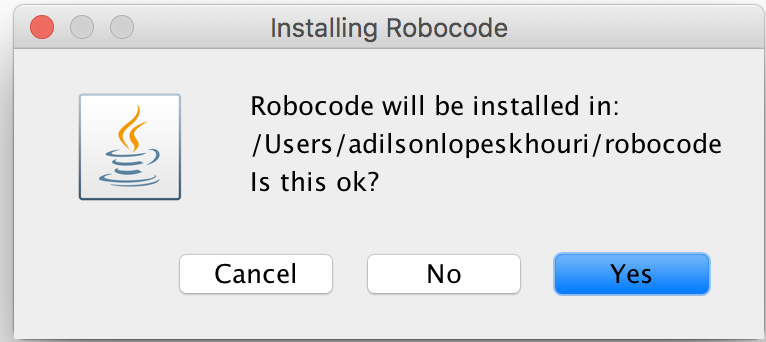
\includegraphics[height=3cm, width = 9cm]{./pic/instalacao01.png}
			\caption{Passo 1 da instalação}
			\label{fig_instalacao01}
		\end{figure}
	\end{block}
\end{frame}


\begin{frame}
	\begin{block}{Instalação}
		 \begin{figure}[!htb]
			\centering	  				
			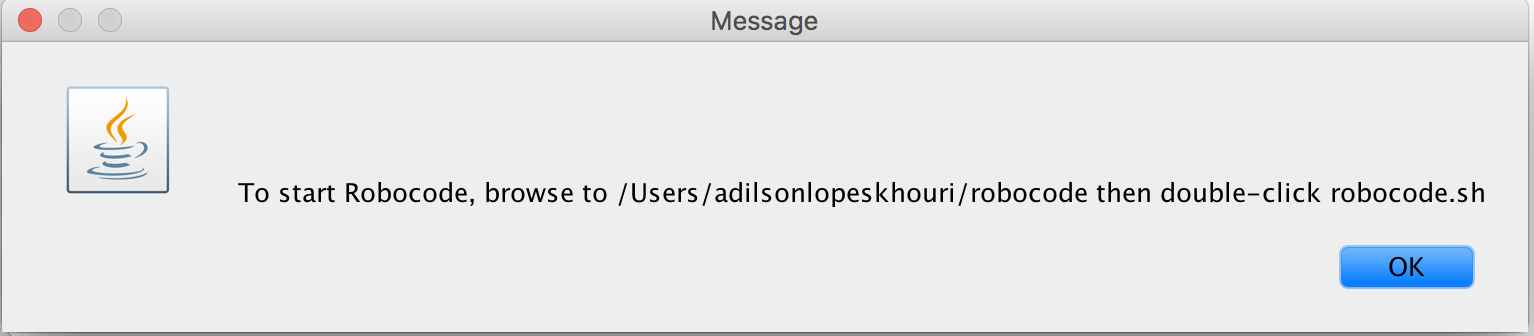
\includegraphics[height=3cm, width = 9cm]{./pic/instalacao02.png}
			\caption{Passo 2 da instalação}
			\label{fig_instalacao02}
		\end{figure}
	\end{block}
\end{frame}



\section{Visão Geral do Jogo}

\begin{frame}
	\begin{block}{Visão Geral do Jogo}
		\begin{itemize}
			\item O campo de batalha funciona com um sistema de coordenadas cartesianas
			\item As rotações possíveis no jogo são sempre em sentido horário			
		\end{itemize}
		
		\begin{figure}[!htb]
			\centering
			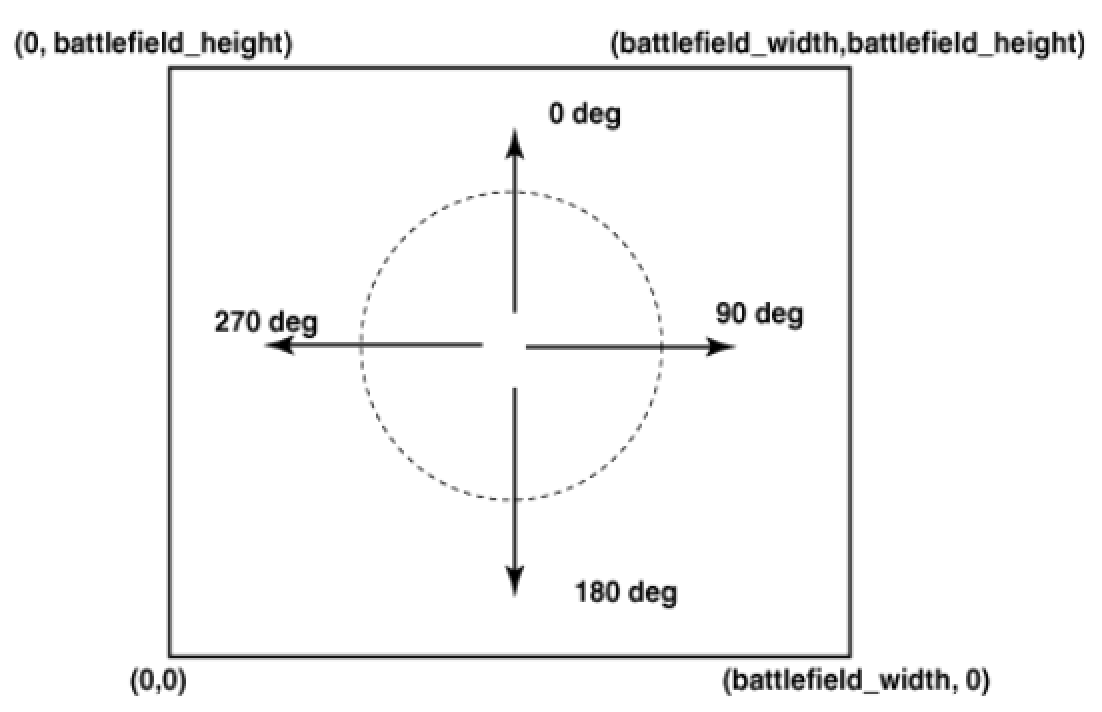
\includegraphics[height=4cm, width = 11cm]{./pic/campoBatalha.png}
			\caption{Campo de batalha baseado em sistema cartesiano  \citep{ROBOWIKI}}
			\label{fig_instalacao03}
		\end{figure}
	\end{block}
\end{frame}


\section{Visão geral do Robô}

\begin{frame}
	\begin{block}{Visão geral do Robô}
		\begin{figure}[!htb]
			\centering	  				
			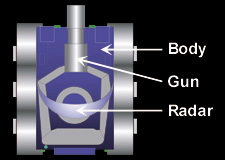
\includegraphics[height=5cm, width = 11cm]{./pic/Anatomy.jpg}
			\caption{Anatomia do robô  \citep{ROBOWIKI}}
			\label{fig_instalacao04}
		\end{figure}
	\end{block}
\end{frame}


\begin{frame}
	\begin{block}{Visão geral do Robô}
		\begin{itemize}
			\item \emph{Body}: Carrega a arma com o radar no topo, o corpo é usado para movimentar o robô para frente/trás e para rotacionar o mesmo
			
			\item \emph{Gun}: Montada no \emph{Body} é responsável por atirar bolas de energia. A arma pode ser rotacionada para: i) direta; ou ii) esquerda

			\item \emph{Radar}: usado para escanear outros robôs durante o movimento do robô, pode ser movimentado para: i) direta; ou ii) esquerda. Esse radar lança o evento:  \emph{onScannedRobot()}  \citep{ROBOWIKI}
						
		\end{itemize}
	\end{block}
\end{frame}


\section{Hands on}

\begin{frame}
	\begin{block}{Hands on}
		\begin{itemize}
			\item Realize o download do arquivo jar aqui: \href{https://sourceforge.net/projects/robocode/files/robocode/1.9.3.4/}{\color{blue}{Source Forge}}  
			
			\item Execute o script:  Users \textbackslash  HOME\_ DIR \textbackslash  robocode \textbackslash robocode.sh
		\end{itemize}
	\end{block}
\end{frame}


\begin{frame}
	\begin{block}{}
		\begin{figure}[!htb]
			\centering	  				
			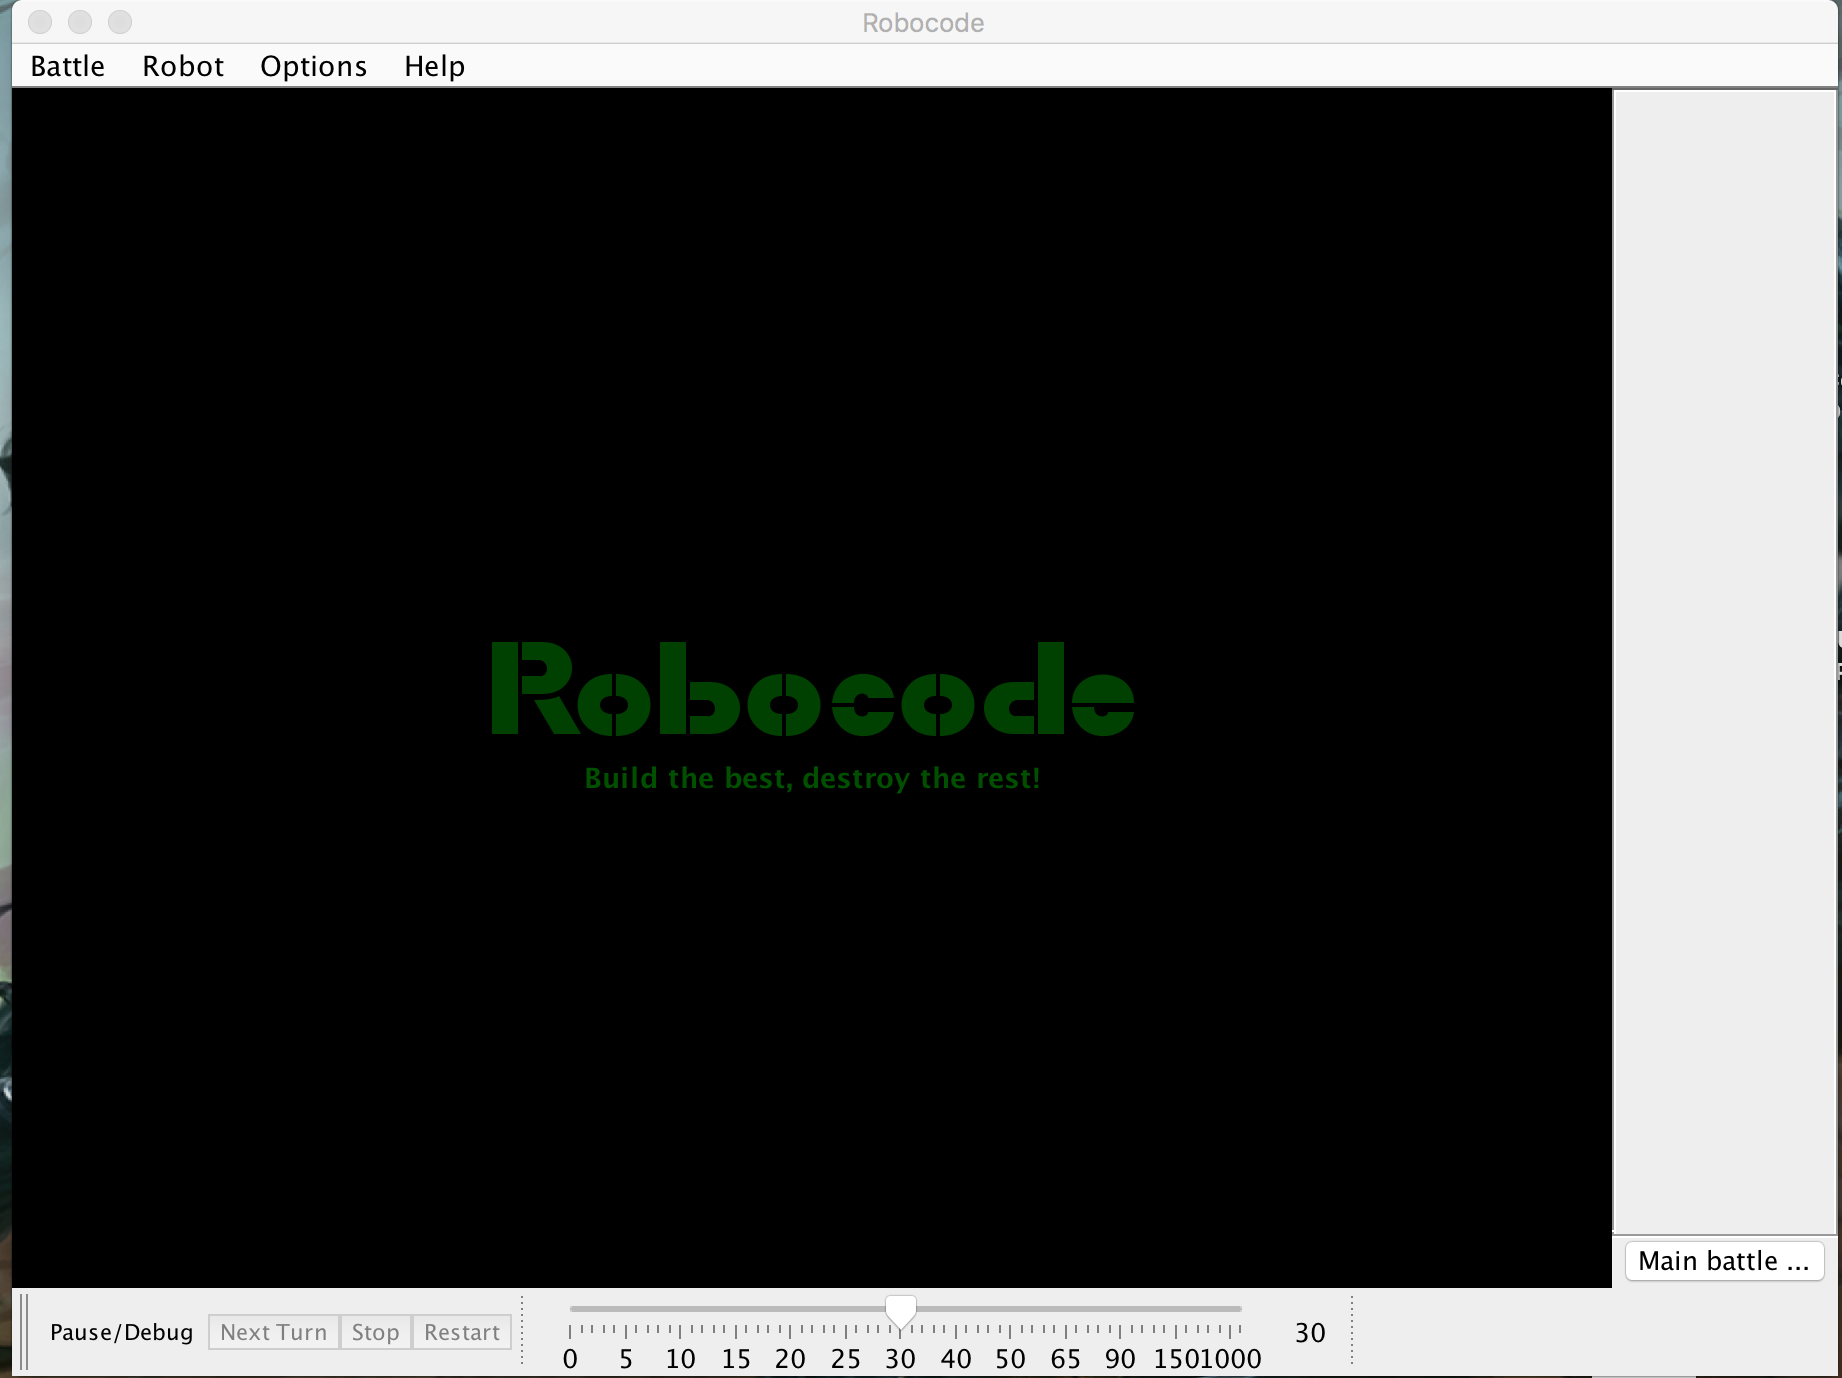
\includegraphics[height=7cm, width = 11cm]{./pic/telaInicial.png}
			\caption{Tela Inicial}
			\label{fig_instalacao04}
		\end{figure}
	\end{block}
\end{frame}


\begin{frame}
	\begin{block}{}
		\begin{figure}[!htb]
			\centering	  				
			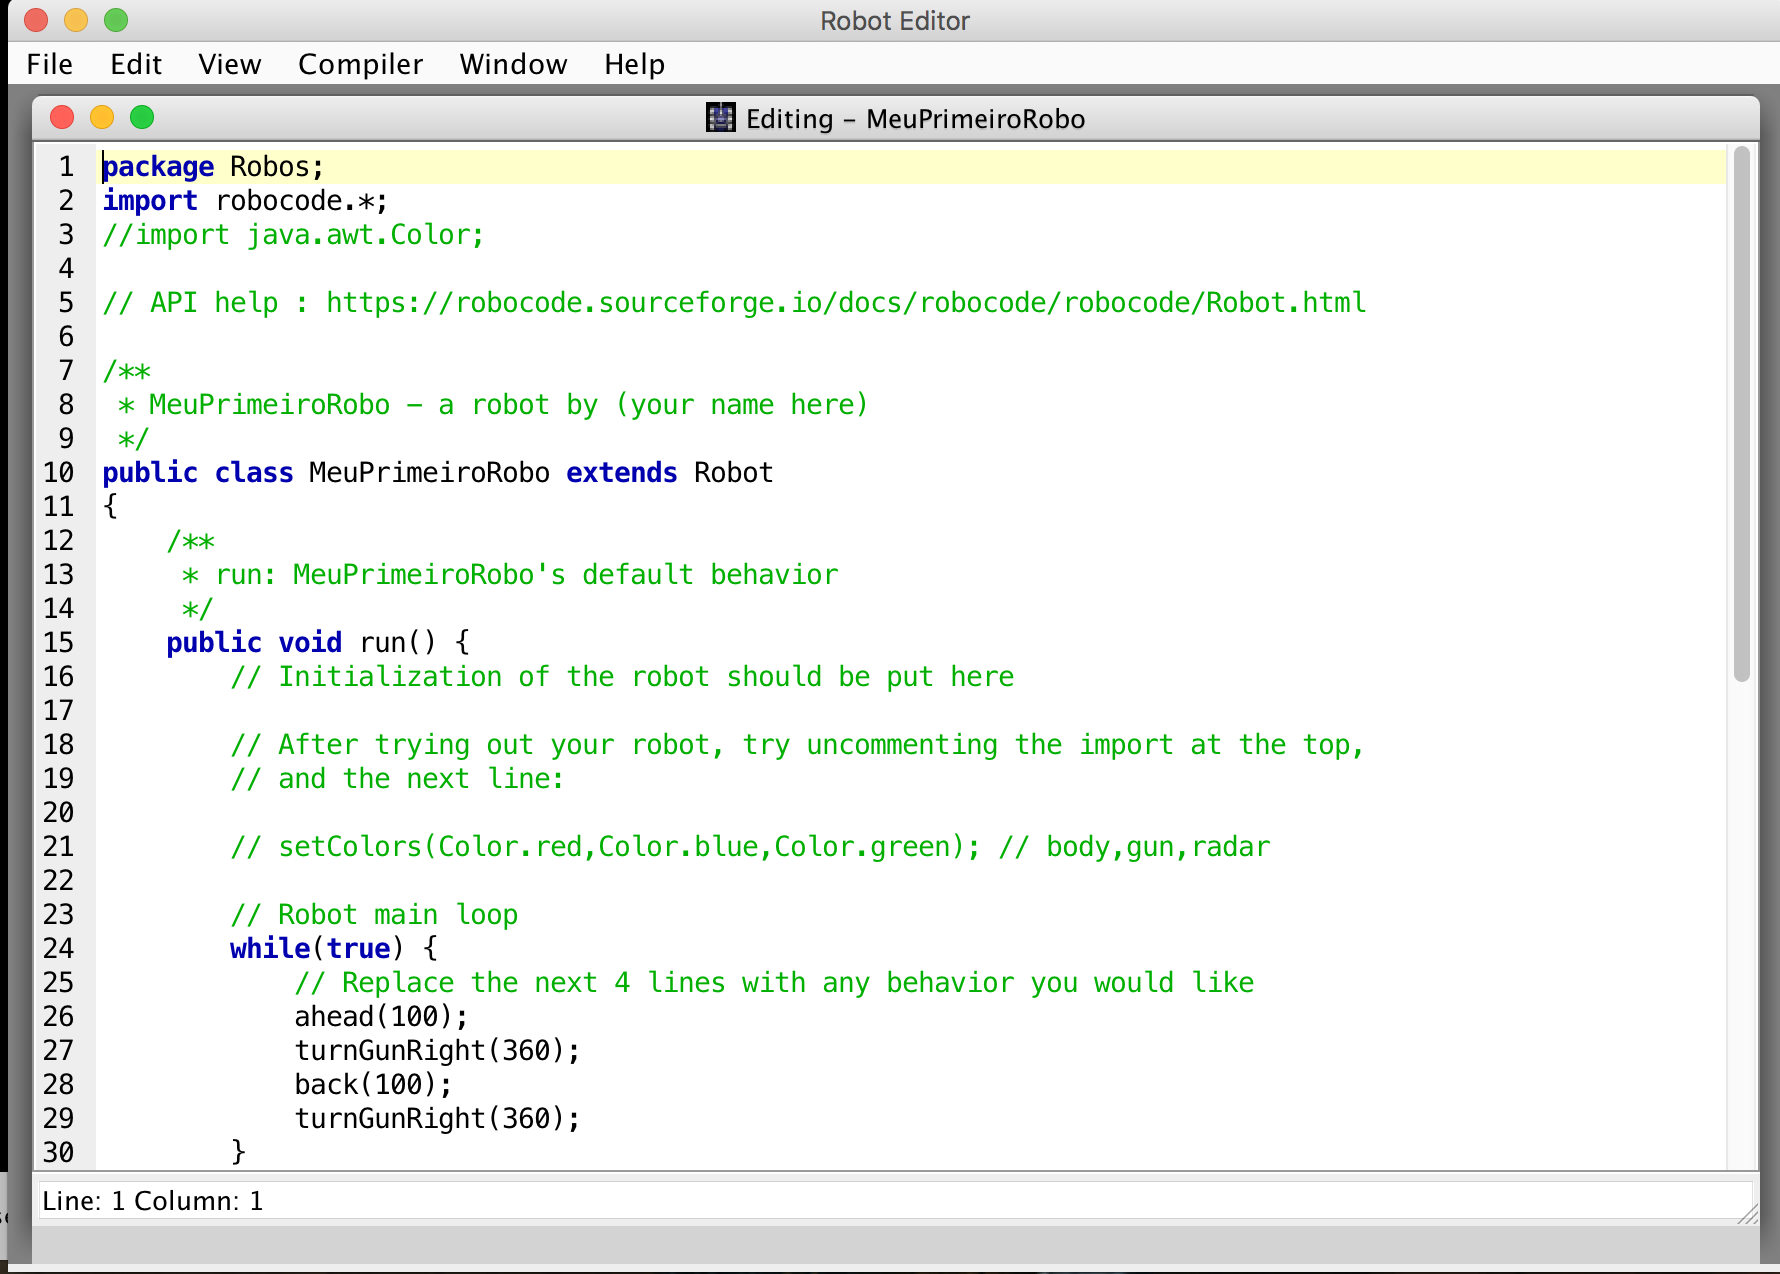
\includegraphics[height=7cm, width = 11cm]{./pic/codigo.png}
			\caption{Tela de codificação}
			\label{fig_instalacao04}
		\end{figure}
	\end{block}
\end{frame}

\begin{frame}
	\begin{block}{}
		\begin{figure}[!htb]
			\centering	  				
			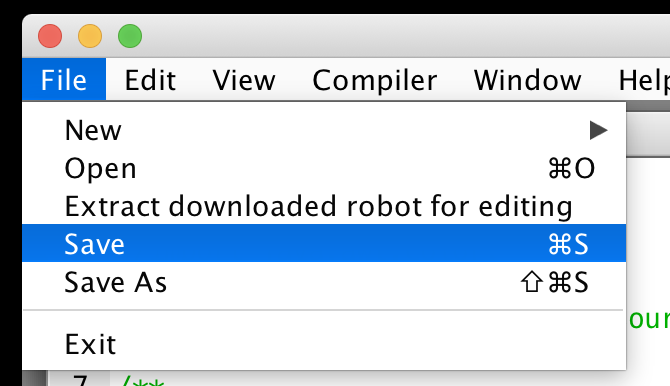
\includegraphics[height=3cm, width = 7cm]{./pic/salvar.png}
			\caption{Tela para salvar}
			\label{fig_instalacao04}
		\end{figure}
	\end{block}
\end{frame}


\begin{frame}
	\begin{block}{}
		\begin{figure}[!htb]
			\centering	  				
			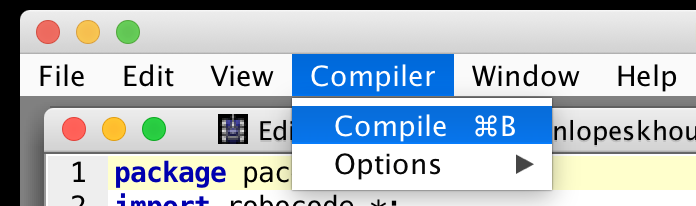
\includegraphics[height=3cm, width = 7cm]{./pic/compilar.png}
			\caption{Tela para compilar}
			\label{fig_instalacao04}
		\end{figure}
	\end{block}
\end{frame}


\begin{frame}
	\begin{block}{}
		\begin{figure}[!htb]
			\centering	  				
			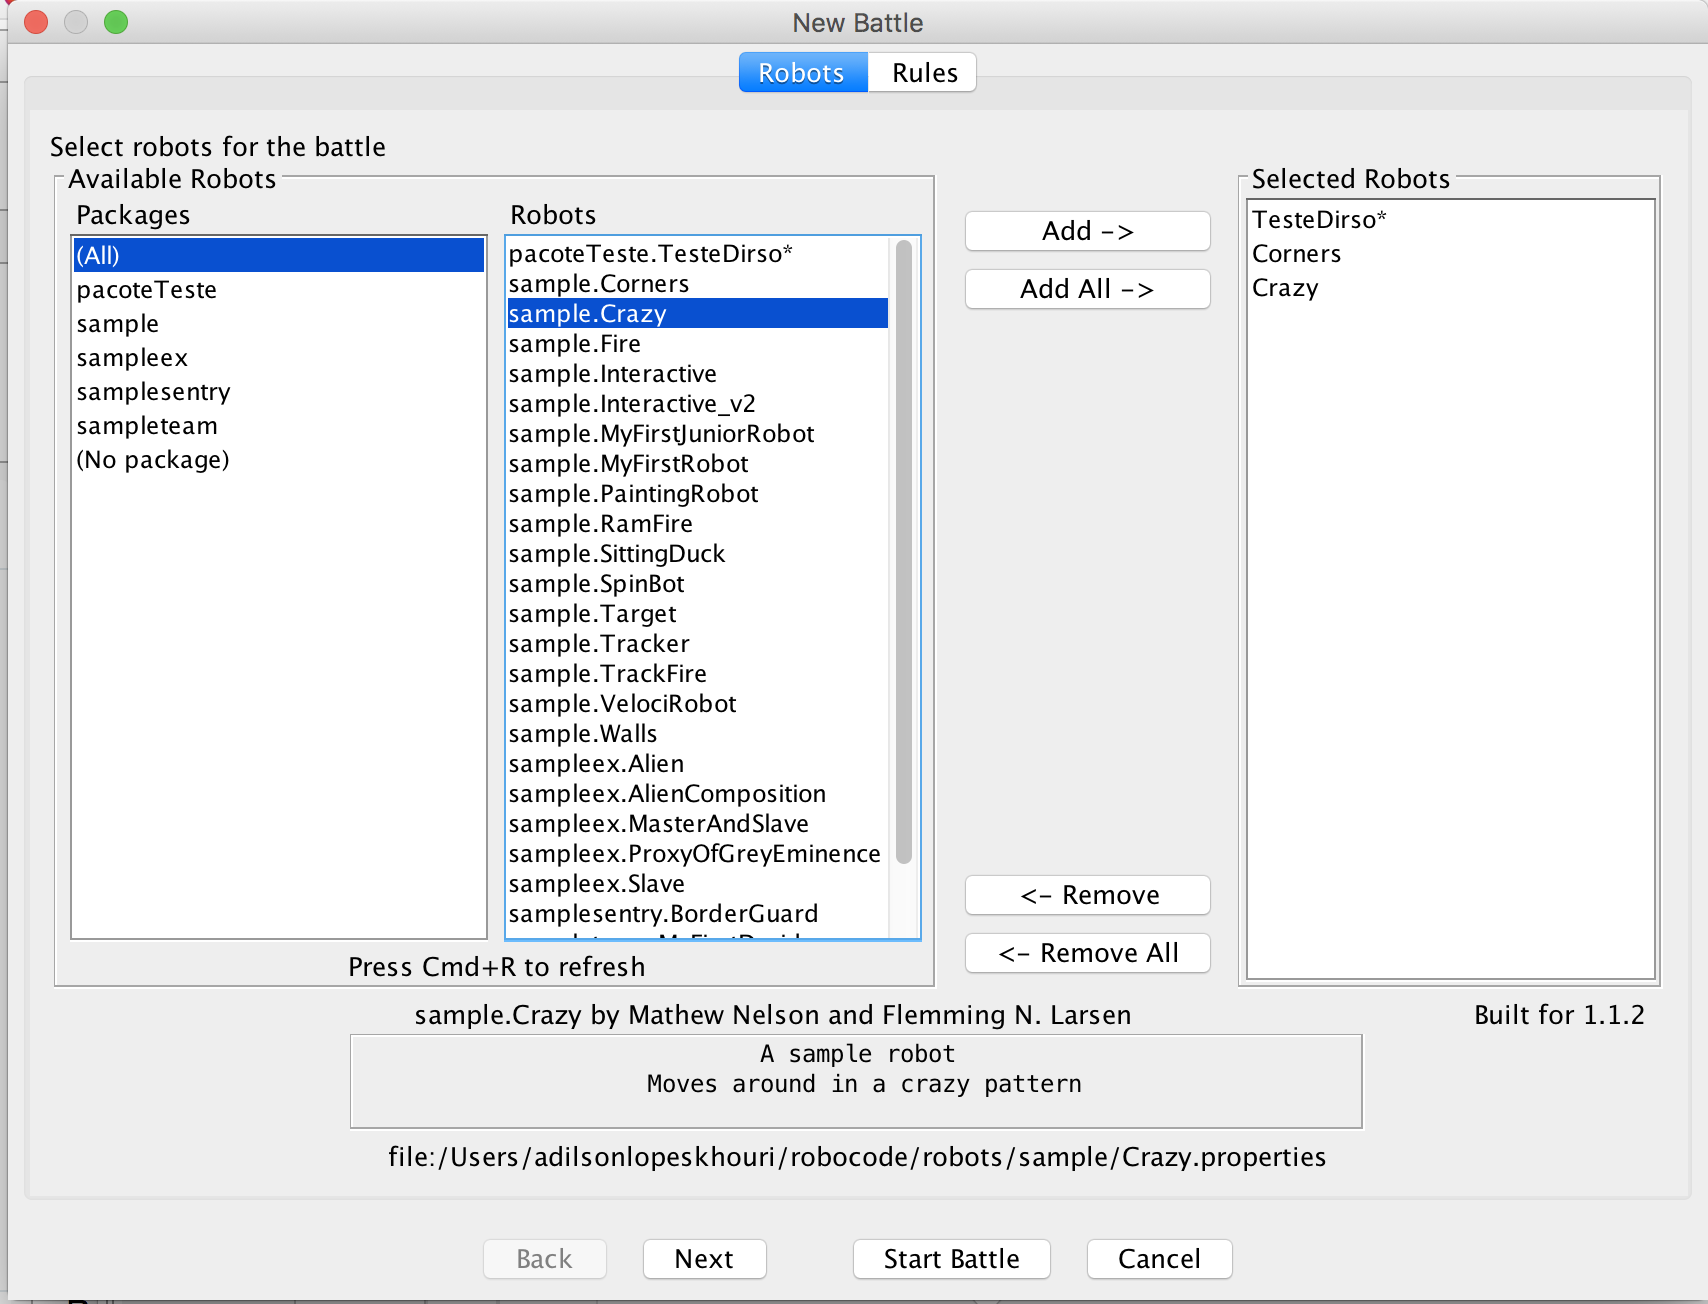
\includegraphics[height=7cm, width = 11cm]{./pic/escolhaRobos.png}
			\caption{Tela para escolher robôs}
			\label{fig_instalacao04}
		\end{figure}
	\end{block}
\end{frame}


\begin{frame}
	\begin{block}{}
		\begin{figure}[!htb]
			\centering	  				
			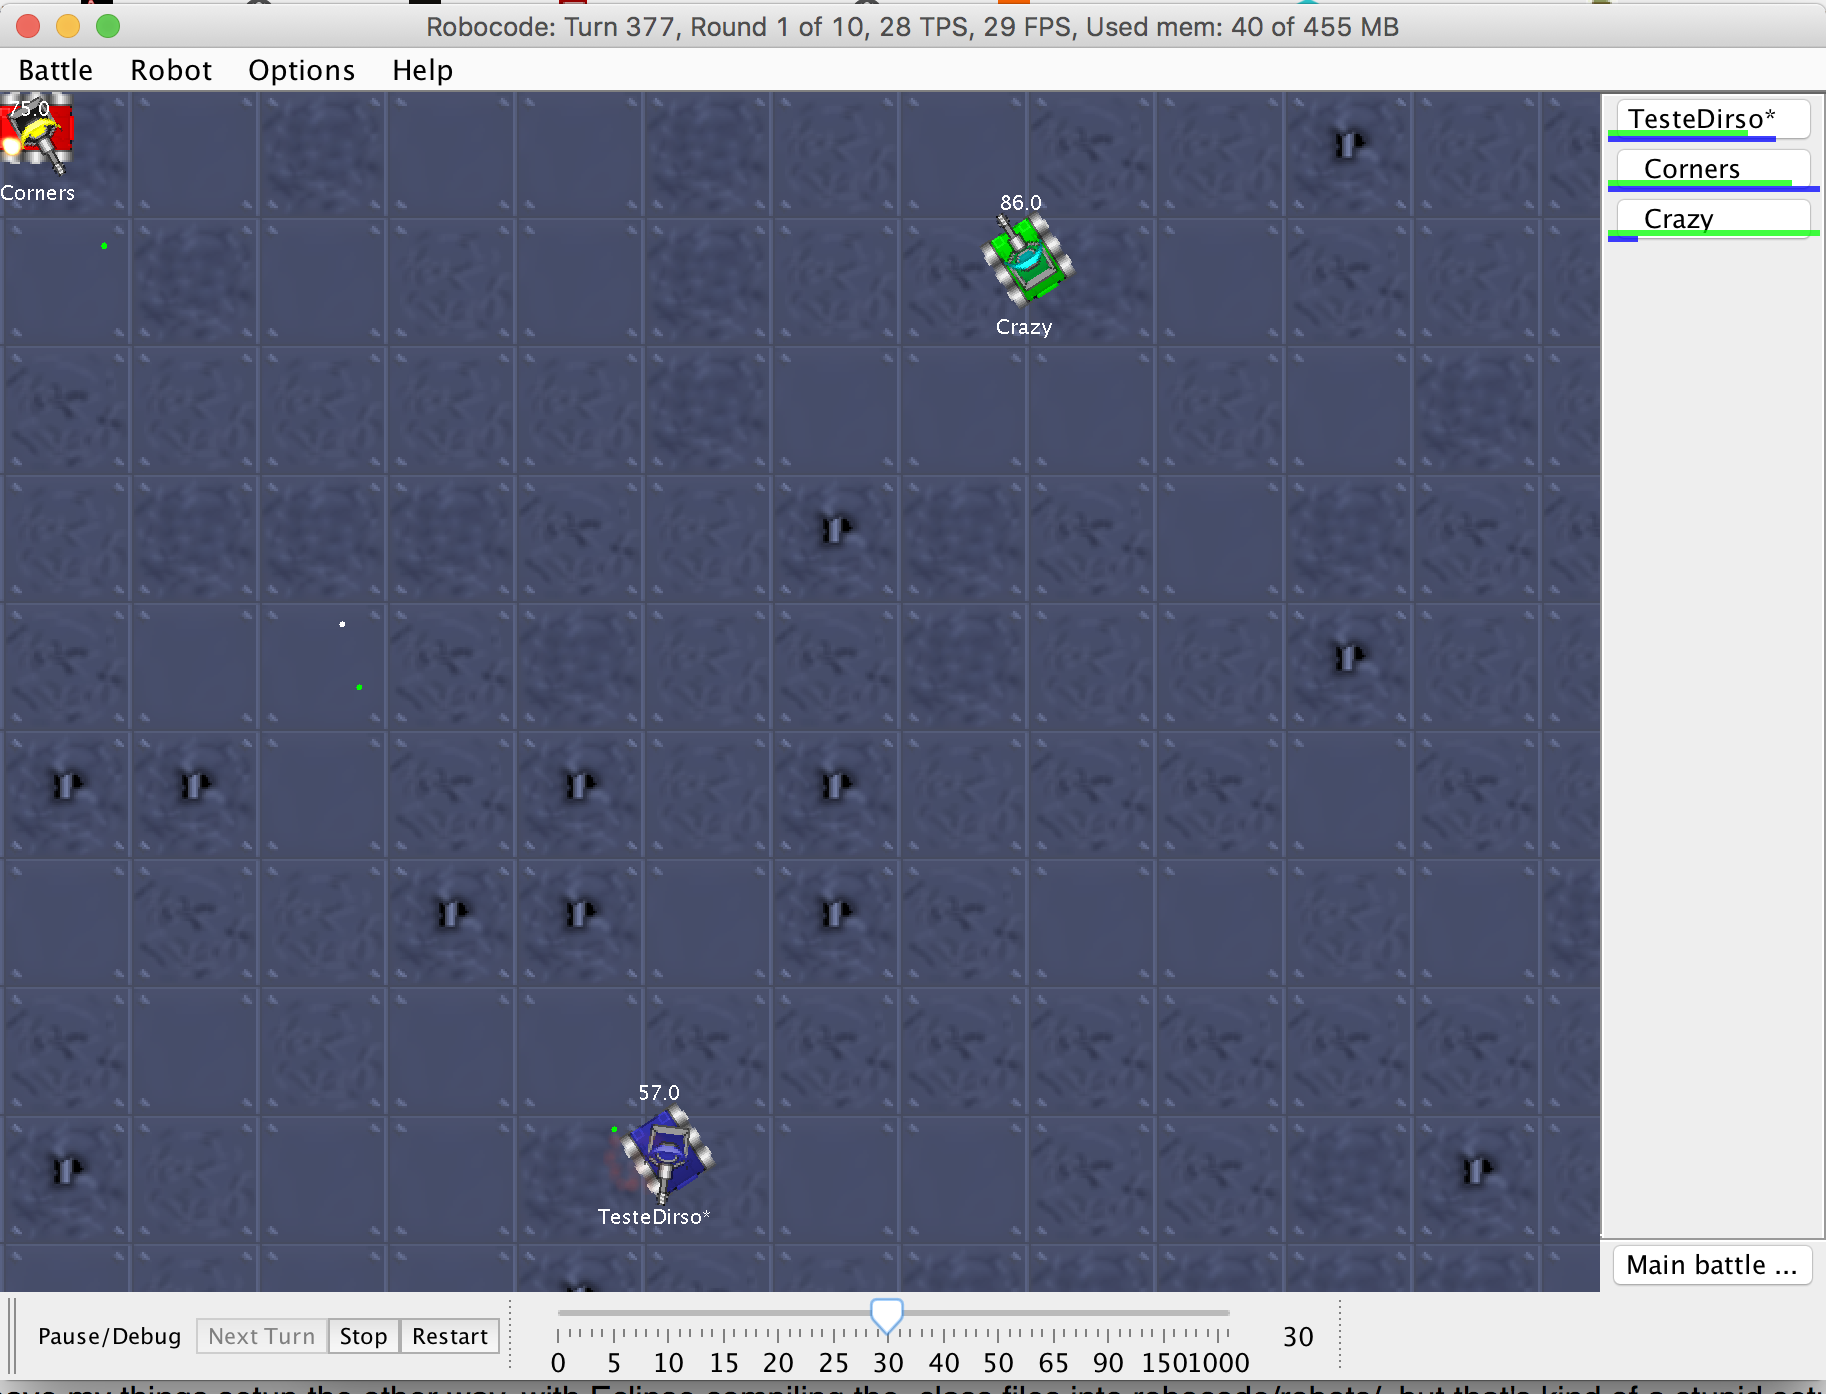
\includegraphics[height=7cm, width = 11cm]{./pic/batalha.png}
			\caption{Campo de batalha}
			\label{fig_instalacao04}
		\end{figure}
	\end{block}
\end{frame}


%// API help : https://robocode.sourceforge.io/docs/robocode/robocode/Robot.html
\section*{Código do robô}

\begin{frame}[fragile]
	\begin{block}{}
		\begin{code}
			
			 \label{code:ClasseRobo}
				\inputminted[linenos,
									fontsize=\footnotesize,
									baselinestretch=1.2,
									framesep=2mm,
									firstline=1,
									lastline=12,
									tabsize=1,
									bgcolor=mygray,									
									frame=lines]
									{java}
									{./secoes/intro/robo.java}
			\captionof{listing}{Classe que representa o robô, herda da classe mãe \emph{Robot}}
			\end{code}
	\end{block}
\end{frame}

\begin{frame}[fragile]
	\begin{block}{}
		\begin{code}
			
			 \label{code:MainWhile}
				\inputminted[linenos,
									fontsize=\footnotesize,
									baselinestretch=1.2,
									framesep=2mm,
									firstline=13,
									lastline=22,
									tabsize=1,
									bgcolor=mygray,									
									frame=lines]
									{java}
									{./secoes/intro/robo.java}
			\captionof{listing}{Laço principal que determina o comportamento do robô}
			\end{code}
	\end{block}
\end{frame}


\begin{frame}[fragile]
	\begin{block}{}
		\begin{code}
			
			 \label{code:Radar}
				\inputminted[linenos,
									fontsize=\footnotesize,
									baselinestretch=1.2,
									framesep=2mm,
									firstline=24,
									lastline=31,
									tabsize=1,
									bgcolor=mygray,									
									frame=lines]
									{java}
									{./secoes/intro/robo.java}
			\captionof{listing}{Evento do radar que identificou um robô}
			\end{code}
	\end{block}
\end{frame}

\begin{frame}[fragile]
	\begin{block}{}
		\begin{code}
			
			 \label{code:onFire}
				\inputminted[linenos,
									fontsize=\footnotesize,
									baselinestretch=1.2,
									framesep=2mm,
									firstline=33,
									lastline=40,
									bgcolor=mygray,									
									tabsize=1,
									frame=lines]
									{java}
									{./secoes/intro/robo.java}
			\captionof{listing}{Evento do seu robô sendo alvejado}
			\end{code}
	\end{block}
\end{frame}


\begin{frame}[fragile]
	\begin{block}{}
		\begin{code}
			
			 \label{code:onHitWall}
				\inputminted[linenos,
									fontsize=\footnotesize,
									baselinestretch=1.2,
									framesep=2mm,
									firstline=42,
									lastline=49,
									tabsize=1,
									bgcolor=mygray,
									frame=lines]
									{java}
									{./secoes/intro/robo.java}
			\captionof{listing}{Evento do seu robô batendo na borda do campo de batalha}
			\end{code}
	\end{block}
\end{frame}


\section{Exercício: Guerra de robôs!}

\begin{frame}
	\begin{block}{Exercício: Guerra de robôs!}
		\begin{itemize}
			\item Codifique seu robô e faremos uma competição entre grupos de alunos!
		\end{itemize}
	\end{block}
\end{frame}
